\documentclass{article}

\title{Big boi words encountered on the weekeepeediah}
\author{Benjamin Bovey - EPFL IC}
\date{Year 2018-2019}

\usepackage{amsmath}
\usepackage{amssymb}
\usepackage{hyperref}

%TikZ
\usepackage{tikz}
\usetikzlibrary{shapes.geometric, shapes.misc, arrows, positioning}
\tikzstyle{big} = [rectangle, minimum width = 3cm, minimum height = 1cm, text centered, text width = 6cm, align = center, draw = black, fill = red!20]
\tikzstyle{medium} = [rounded rectangle, minimum width = 3cm, minimum height = 1cm, text centered, text width = 6cm, align = center, draw = black]
\tikzstyle{arrow} = [thick, ->, > = stealth]


\begin{document}
\maketitle
\section*{Introduction}
This document's purpose is to sort of organize the abstract terms often encountered while browsing mathematics articles on wikipedia. It will surely contain a bunch of errors in terms of strict definitions. I hope to improve that as time goes.

\section{Algebraic structures}
\subsection{General understanding}
Some examples of algebraic structures often encountered on Wikipedia are fields, magmas, groups, rings... They are all derived from sets, more precisely from adding some kind of structure to those sets, that is, equipping them with operations. \\
Even more precisely, it would seem that the words "algebraic structure" are independent on the set; that is, an algebraic structure is a collection of operations that a set, called the \emph{underlying set} or \emph{carrier set}, can be equipped with. It also seems that the operations of an algebraic structure must be \emph{finitary}, which means that they have a finite amount of operands. \\
According to \href{http://math.wikia.com/wiki/Algebraic_structure}{the math wikia}, "an algebraic structure is one or more sets combined with one or more operations, and optionally with a relation [...] that satisfies a given set of properties". Here the definition seems to also regard the set which is given these operations. \\

The goal of the below flowchart is to give a sort of general view of how the main types of algebraic structures relate to and differ from each other. For vocabulary, refer to the next subsections. This flowchart's organization and content are greatly inspired by the \href{http://math.wikia.com/wiki/Algebraic_structure}{wikia article on algebraic structures}.

%--------------------------
\begin{figure}
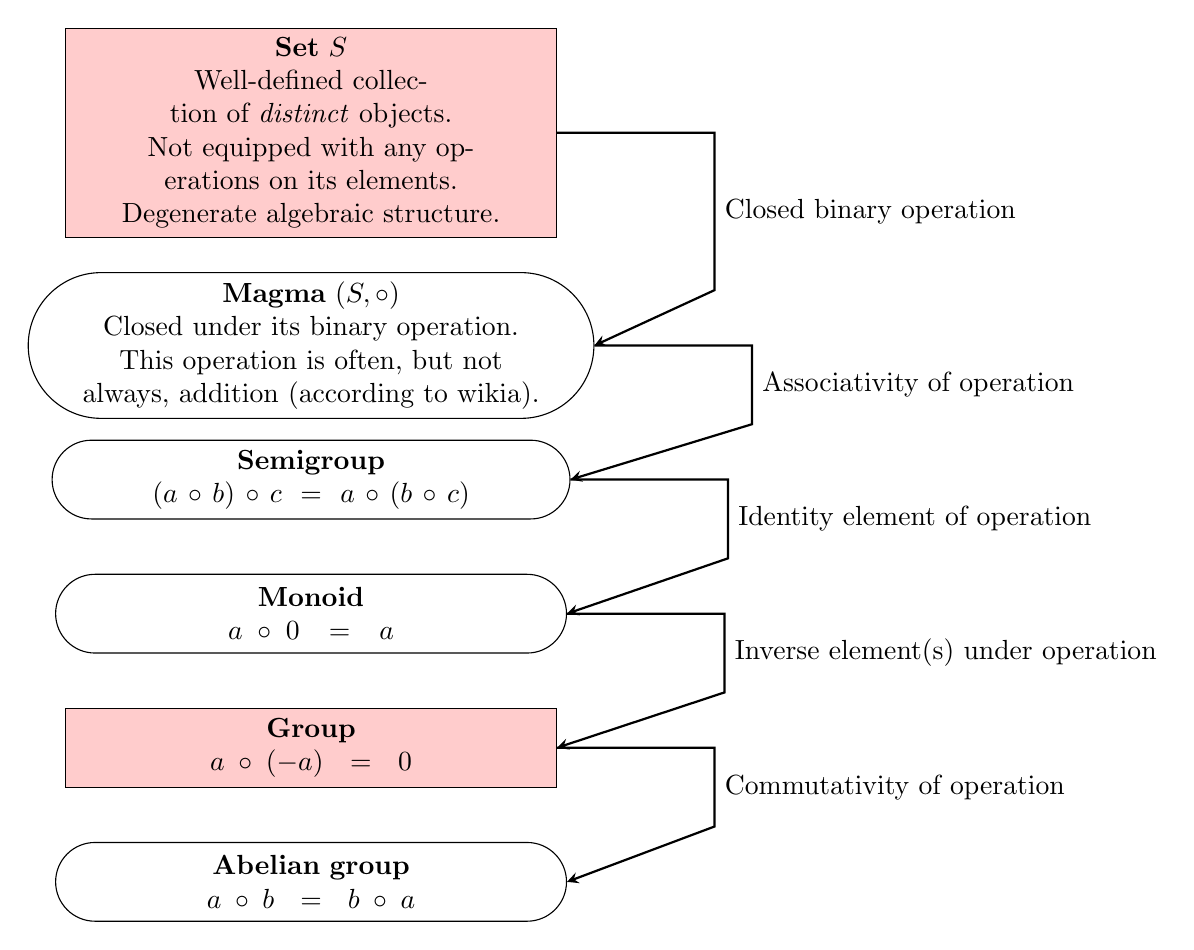
\begin{tikzpicture}[node distance = 20pt]

%NODES
\node (set) [big] {\textbf{Set} \(S\) \\ Well-defined collection of \emph{distinct} objects. \\ Not equipped with any operations on its elements. \\ Degenerate algebraic structure.};
\node (magma) [medium, below of = set, yshift = -2cm] {\textbf{Magma} \((S, \circ)\) \\ Closed under its binary operation. This operation is often, but not always, addition (according to wikia).};
\node (semigroup) [medium, below of = magma, yshift = -1cm] {\textbf{Semigroup} \\ \((a \circ b) \circ c = a \circ (b \circ c)\)};
\node (monoid) [medium, below of = semigroup, yshift = -1cm] {\textbf{Monoid} \\ \(a \circ 0 = a\)};
\node (group) [big, below of = monoid, yshift = -1cm] {\textbf{Group} \\ \(a \circ (-a) = 0\)};
\node (abeliangroup) [medium, below of = group, yshift = -1cm] {\textbf{Abelian group} \\ \(a \circ b = b \circ a\)};

%ARROWS
\draw [arrow] (set.east) -- ++(2, 0) -- node[anchor = west]{Closed binary operation} ++(0, -2	) -- (magma.east);
\draw [arrow] (magma.east) -- ++(2, 0) -- node[anchor = west]{Associativity of operation} ++(0, -1) -- (semigroup.east);
\draw [arrow] (semigroup.east) -- ++(2, 0) -- node[anchor = west]{Identity element of operation} ++ (0, -1) -- (monoid.east);
\draw [arrow] (monoid.east) -- ++(2, 0) -- node[anchor = west]{Inverse element(s) under operation} ++(0, -1) -- (group.east);
\draw [arrow] (group.east) -- ++(2, 0) -- node[anchor = west]{Commutativity of operation} ++(0, -1) -- (abeliangroup.east);

\end{tikzpicture}
\caption{The first main types of algebraic structures.}
\end{figure}
%--------------------------
\subsection{Operations}
An operation is similar to a function, in that it takes input and gives output. It is, however, a lower-level and more general term than "function".
\subsection{Notation}
Since we're talking about operations themselves on an abstract level, we have to be careful when considering notation. The notation commonly used to talk about, for example, a magma, would be to put the set and the operation that we give it in a 2-tuple: \((G, \circ)\) would be the magma with underlying set \(G\), and binary operation \(\circ\). However, \(\circ\) does \textbf{NOT} necessarily mean function composition in this context - it could, but it could also be any other operation: remember that we are talking about the concept of an operation itself, not any specific operation. We simply need a symbol to represent that operation, in this case, it is \(\circ\). But it could be anything: \((G, +)\), for example. \\
\emph{Note}: this also means that in the diagram above, when introducing the inverse element, the \(-\) sign in \(-a\) is not to be interpreted in the "classical" sense of negative, or of minus.
\subsection{Arity}
The arity of an operation is the amount of operands that the operation takes. Here are some examples for relations with low arity:
\begin{itemize}
	\item \textbf{Unary:} On a number, we could have the inverse, opposite, square root, square... On a boolean, we could have negation. On a bit string, we could have negation as well. On a function, we could have derivation, integration, inverse...
	\item \textbf{Binary:} There are a ton of these. On two numbers, we could have addition, substraction, multiplication, division, raising one to the power of the other... Addition and multiplication are found over many sets.
	\item \textbf{Ternary:} We'll find some examples later
\end{itemize}
\subsection{Closure}
A set is said to be closed \emph{under a certain operation} if applying this operation to elements of the set results in an output that is an element of the set. \\

A set is said to be closed \emph{under a collection of operations} if it is closed under each of the operations individually. \\

For example, the set of natural numbers \(\mathbb{N}\) is closed under addition: any positive integer added to another positive integer will result in a positive integer. However, \(\mathbb{N}\) is not closed under substraction: for example, \(3 - 4\) is not contained in \(\mathbb{N}\), even though \(3\) and \(4\) are. Similarly, \(\mathbb{Z}\) is not closed under division. The set containing only zero, \(\{0\}\), is closed under addition, substraction and multiplication. \\

Now, there seems to be a second meaning to the term "closure". That is, when a set \(S\) is \emph{not} closed under some operations, one can find the smallest set containing \(S\) that is closed under these operations. This smallest closed set is then called \emph{the closure of \(S\) under these operations}. \\

So the closure of a set \(S\) under operation \(\circ\) can be either of the following:
\begin{itemize}
	\item the logical proposition "\(S\) is closed under \(\circ\)" and false otherwise; that is, the "property of being closed under \(\circ\)"
	\item if the above logical proposition does not hold, the closure is the smallest subset containing \(S\) that is closed under \(\circ\)
\end{itemize}

We could therefore state that \(\mathbb{N}\) is not closed under substraction, and that the closure of \(\mathbb{N}\) under substraction is \(\mathbb{Z}\).




\end{document}